%-----------------------------------------------------------------------------%
\chapter{HASIL PENELITIAN DAN PEMBAHASAN}
%-----------------------------------------------------------------------------%

%
\vspace{4.5pt}
\begin{flushleft}
    \begin{justify}
        \section{Hasil Penelitian}
        \subsection{Hasil Observasi}
        Peneliti mengamati kebutuhan sensor dan kontrol yang sering diaplikasikan pada lahan untuk kebutuhan pembuatan aplikasi KEBUNQ. Didapat data sebagai berikut.\\
        \subsubsection{Sensor} 
        Berikut beberapa sensor yang biasa digunakan pada lahan pertanian yang perlu dicantumkan ke aplikasi KEBUNQ :
        \begin{enumerate}
            \item Suhu
            \item \emph{Humidity}
            \item Intensitas Cahaya
            \item Suhu Tanah
            \item \emph{Humidity} Tanah
            \item pH Tanah
            \item Suhu Air
            \item TDS (ppm meter)
            \item pH Air\\
        \end{enumerate}
        \subsubsection{Kontrol}
        Berikut beberapa kontrol yang biasa digunakan pada lahan pertanian yang perlu dicantumkan ke aplikasi KEBUNQ :
        \begin{enumerate}
            \item \emph{Mist} 
            \item \emph{Sprinkler} 
            \item \emph{Fan} 
            \item \emph{Valve} 
            \item \emph{Drip} 
            \item Pompa 
            \item Lainnya (\emph{Customize})\\
        \end{enumerate}
        % \caption{Gambar Observasi}
        \subsection{Hasil Penerapan RAD}
        \subsubsection{Pemodelan Bisnis}
        Berdasarkan hasil analisa ditentukan bahwa aplikasi KEBUNQ dirancang untuk satu jenis pengguna. Sehingga tidak terdapat level pengguna pada akses aplikasi.
        Berikut analisa kebutuhan pengguna
        \begin{enumerate}
            \item Pengguna harus melakukan login
            \item Pengguna dapat melihat daftar dan status nyala alat
            \item Pengguna dapat melihat detail alat yang terdiri dari data sensor dan kontrol yang tersedia
            \item Pengguna dapat melakukan kontrol pada alat yang dipilih
            \item Pengguna dapat melakukan setting automatis pada suatu kontrol yang tersedia mode automatisnya\\
        \end{enumerate}
       
        \subsubsection{Pemodelan Data}
        \begin{figure}[ht]
            \centering
            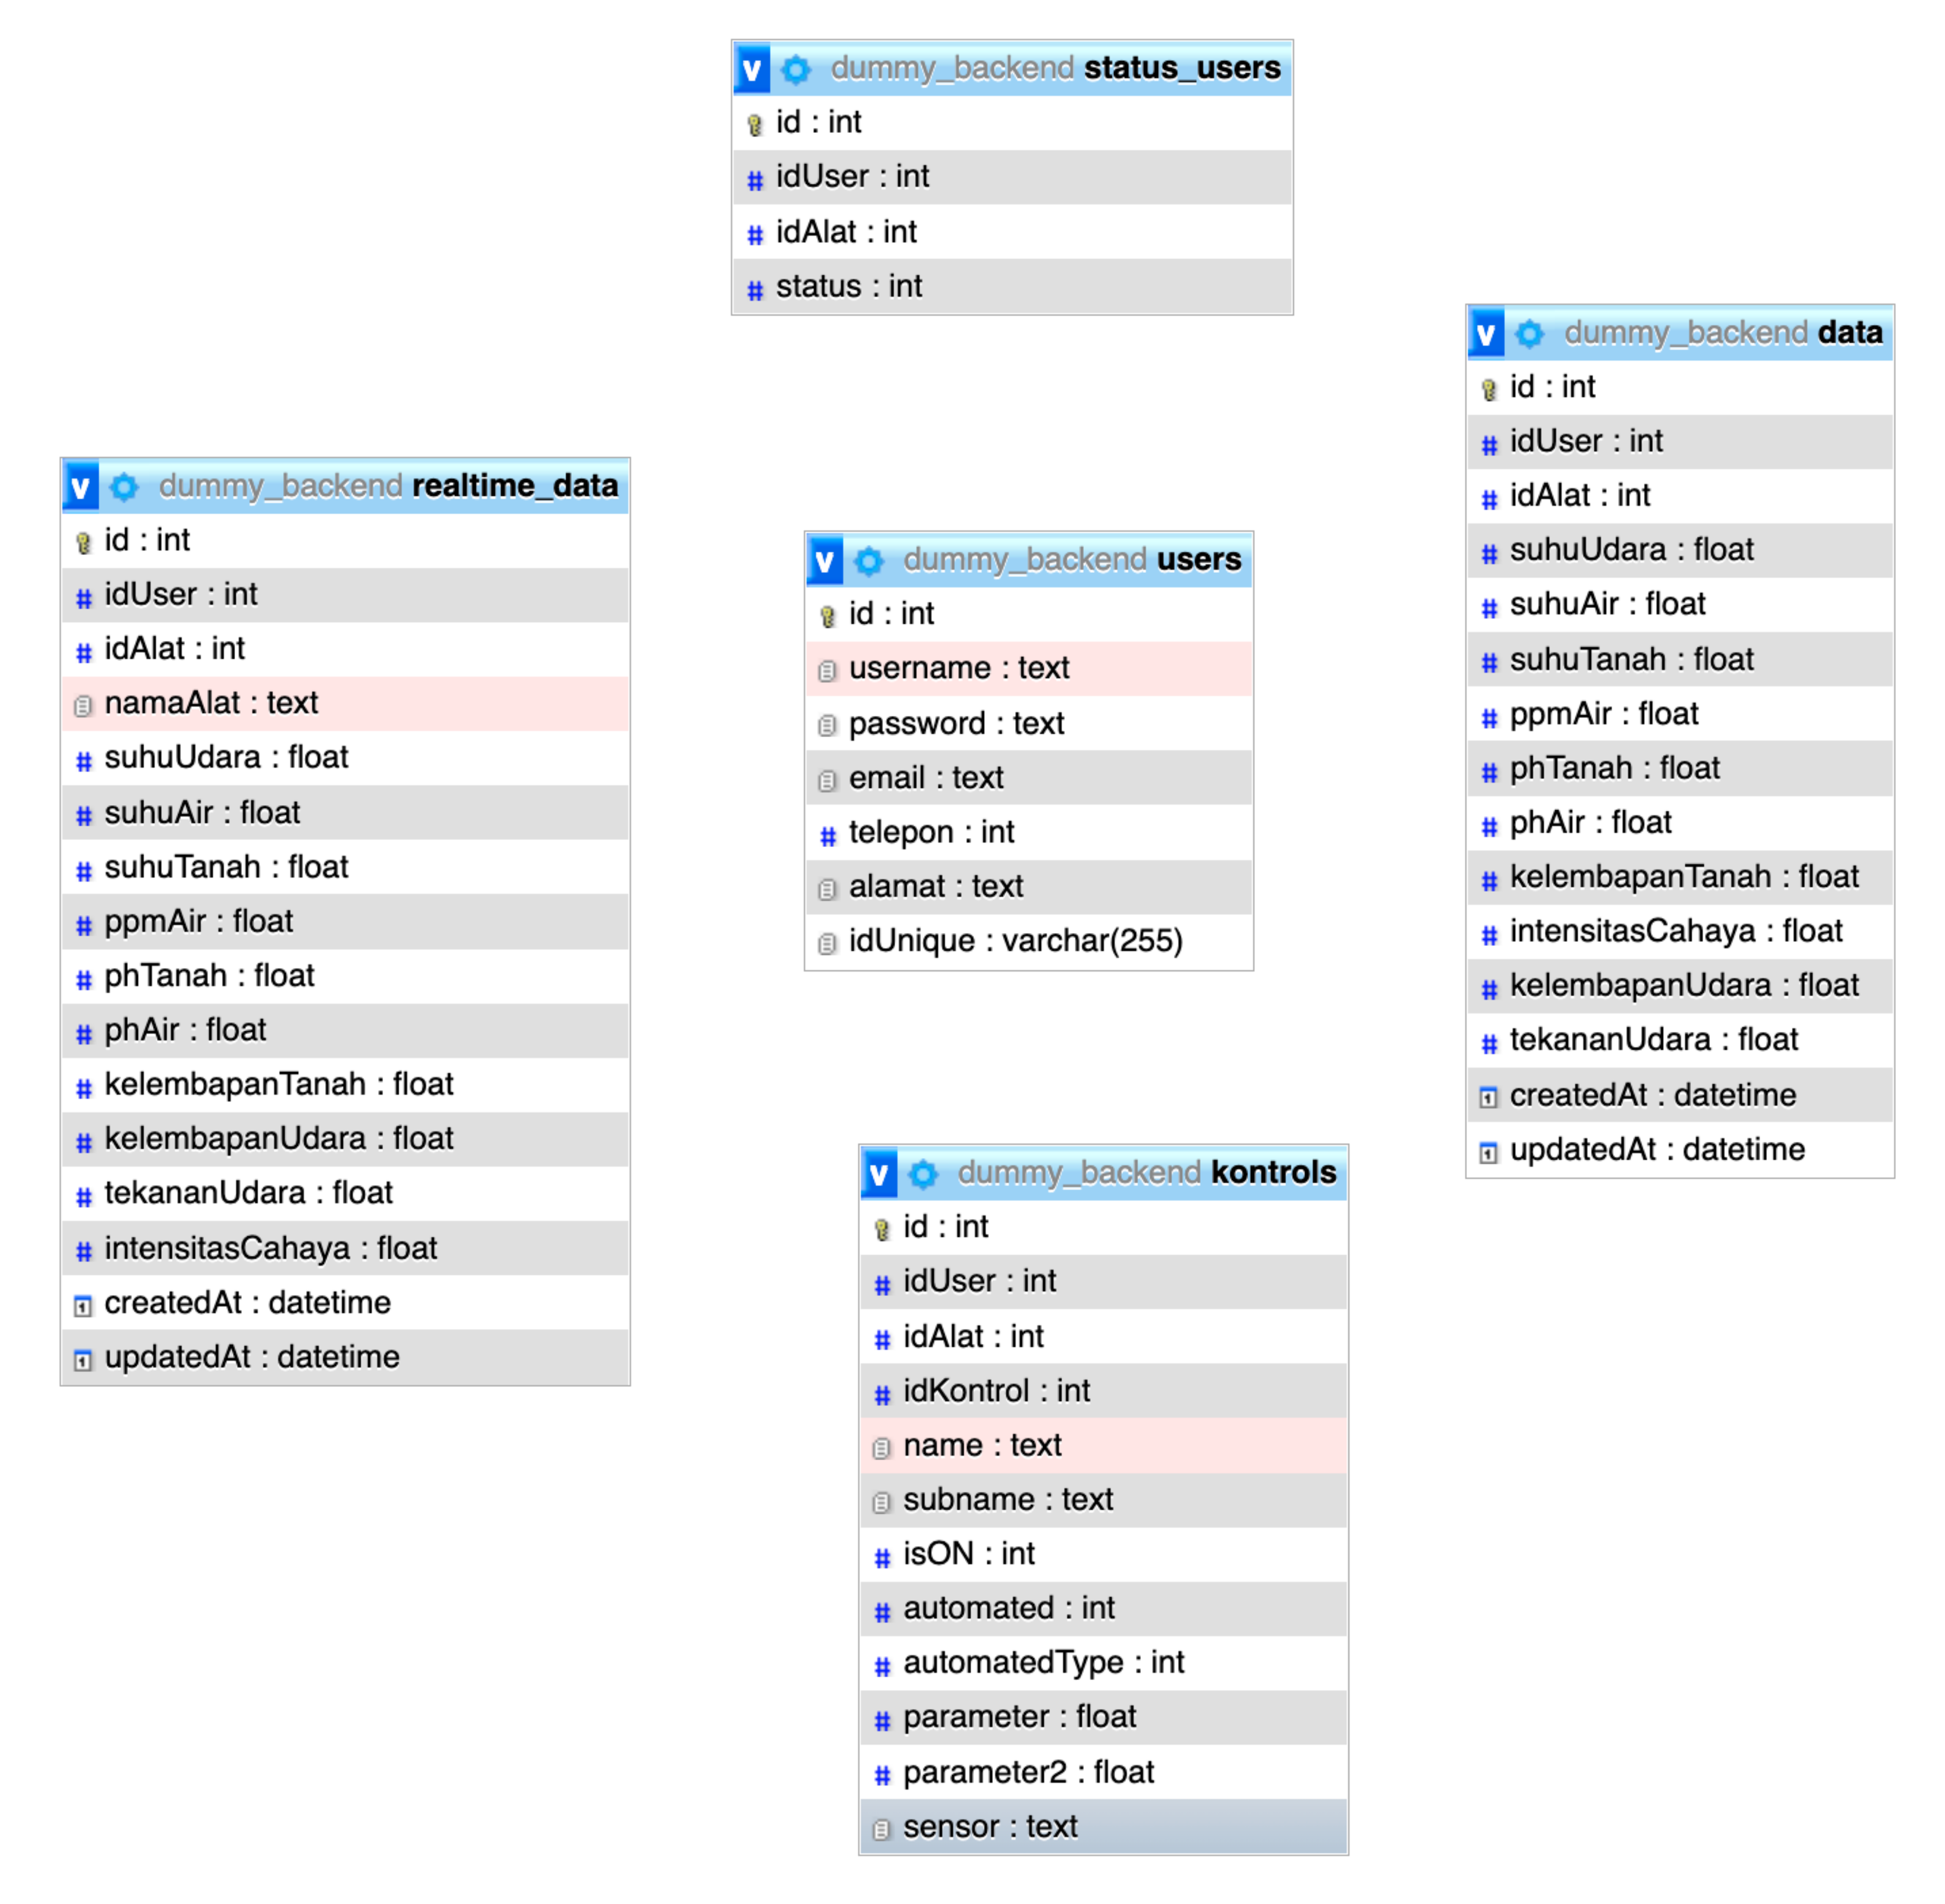
\includegraphics[width=8cm]{images/database.png}
            \caption{Skema Tabel \textit{Database}}
        \end{figure}
        \noindent \\Setelah dilakukan tahap pemodelan bisnis, maka didapatkan skema \emph{database} yang dirancang seperti gambar 4.1 di atas. \emph{Database} terdiri dari lima tabel yakni (1) tabel data, digunakan untuk menyimpan data time series dari nilai sensor yang ada pada alat, 
        (2) tabel kontrols, digunakan untuk menyimpan dan mendefinisikan kontrol yang dimiliki, 
        (3) tabel realtime\_data, digunakan untuk menyimpan data realtime sensor dan kontrol,
        (4) tabel status\_users, digunakan untuk menyimpan status alat apakah \emph{online} atau \emph{offline},
        dan (5) tabel users, digunakan untuk menyimpan data user. Setelah skema \emph{database} difinalisasi, 
        maka dilakukan pembuatan \emph{Application Programming Interface} (API) dan konfigurasi server yang dalam bagian ini 
        pengerjaan bukan dilakukan oleh peneliti namun oleh anggota lain dalam proyek. 
        Sehingga akhirnya didapat beberapa API (\emph{dummy}) sebagai berikut dengan \emph{endpoint} yang dirahasiakan demi keamanan aplikasi :
            \begin{itemize}
                \item API login\\
                http://47.89.212.89/dummyBackend/(\emph{endpoint})
                \item API \emph{Summary Data} dari pengguna\\
                http://47.89.212.89/dummyBackend/data/(\emph{endpoint})
                \item API data \emph{realtime}\\
                http://47.89.212.89/dummyBackend/data/mobile/(\emph{endpoint})
                \item API data kontrol\\
                http://47.89.212.89/dummyBackend/kontrol/(\emph{endpoint})
                \item API data ikon\\
                http://47.89.212.89/dummyBackend/(\emph{endpoint}) \\
                (\emph{endpoint} berada pada API data \emph{realtime})
                \item API status alat\\
                http://47.89.212.89/dummyBackend/status/(\emph{endpoint})
                \item API update kontrol\\
                http://47.89.212.89/dummyBackend/kontrol/(\emph{endpoint})
            \end{itemize}
        API ini digunakan oleh peneliti dalam tahap pembuatan aplikasi \emph{mobile} KEBUNQ sebagai penghubung antara aplikasi dengan \emph{database server}.\\
        

        

        \subsubsection{Pemodelan Proses}
        \begin{enumerate}[label=\alph*.]
            \item \textit{Use Case}
            \textit{Use case} perancangan aplikasi mobile KEBUNQ BPP Lampung yang dirancang setelah menganalisa tahap pemodelan bisnis dan 
            pemodelan data dapat dilihat pada Gambar 4.2
            \begin{figure}[ht]
                \centering
                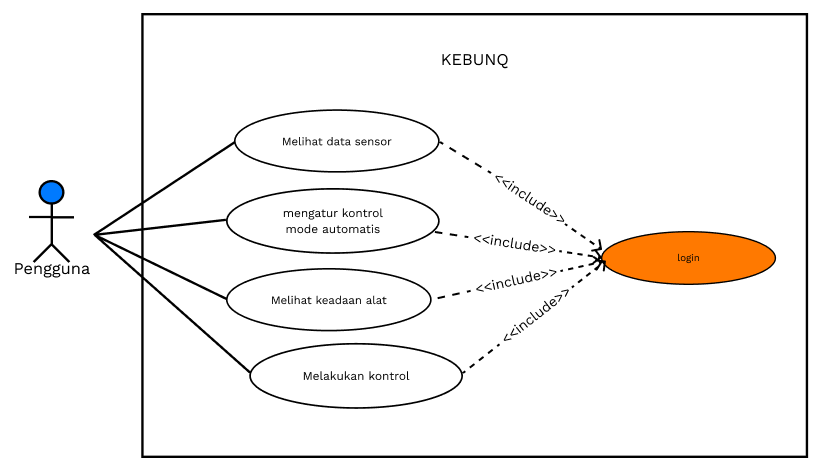
\includegraphics[width=10cm]{images/bab 4/use-case-user.png}
                \caption{\textit{Use Case Diagram}}
            \end{figure}
            \item \textit{Sequence Diagram}
            \begin{figure}[ht]
                \centering
                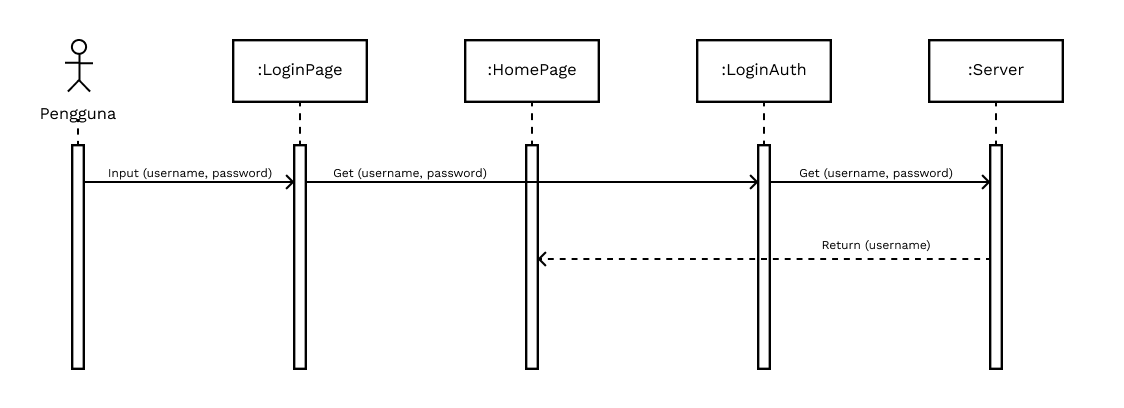
\includegraphics[width=12cm]{images/bab 4/Sequence login.png}
                \caption{\textit{Sequence Diagram Login}}
            \end{figure}
            \begin{figure}[ht]
                \centering
                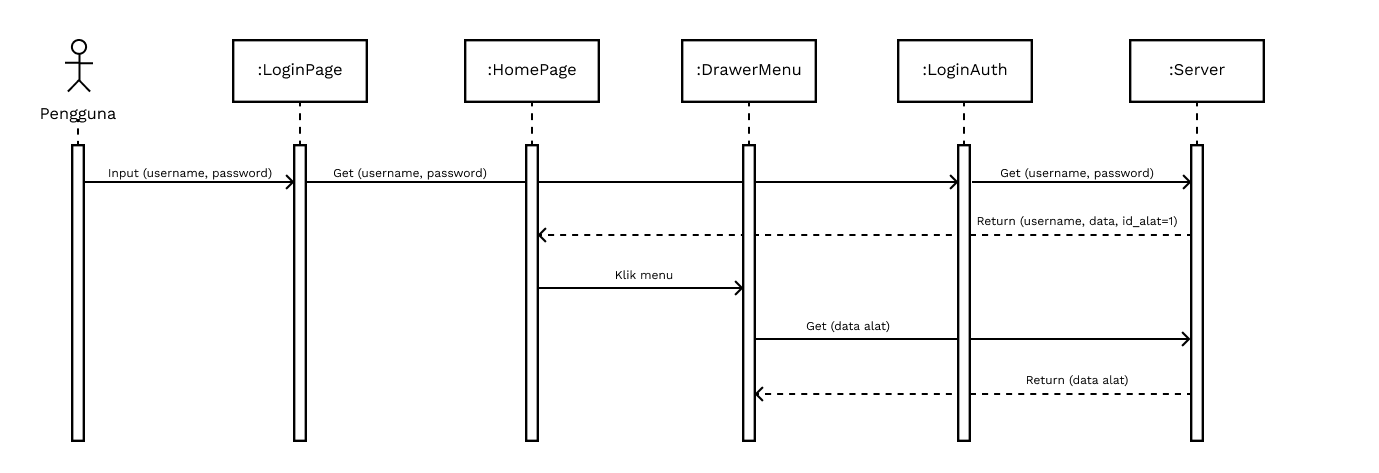
\includegraphics[width=12cm]{images/bab 4/buka menu alat.png}
                \caption{\textit{Sequence Diagram} Melihat Menu / Alat}
            \end{figure}
            \vspace{5cm}
            \begin{figure}[ht]
                \centering
                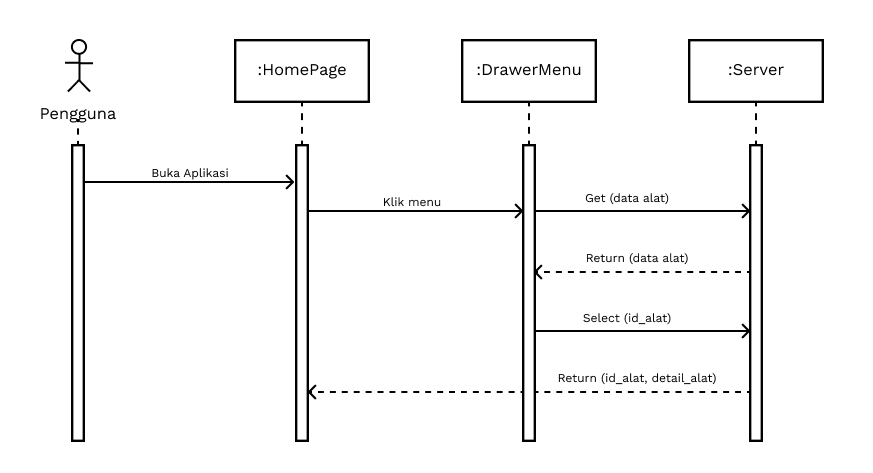
\includegraphics[width=14cm]{images/bab 4/Sequence buka detail alat.png}
                \caption{\textit{Sequence Diagram} Melihat Detail Alat}
            \end{figure}

            \begin{figure}[ht]
                \centering
                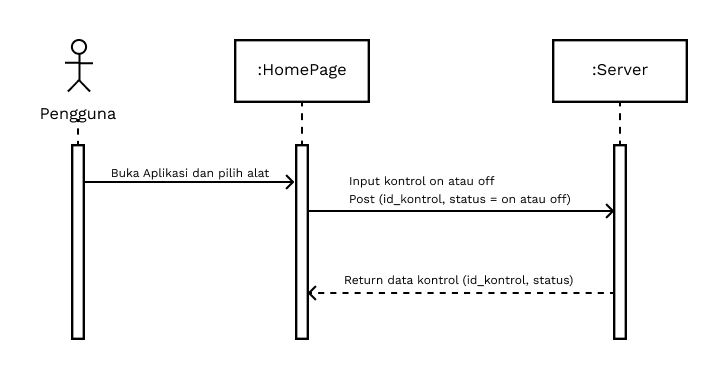
\includegraphics[width=14cm]{images/bab 4/Sequence kontrol.png}
                \caption{\textit{Sequence Diagram} Melakukan Kontrol}
            \end{figure}
            \begin{figure}[ht]
                \centering
                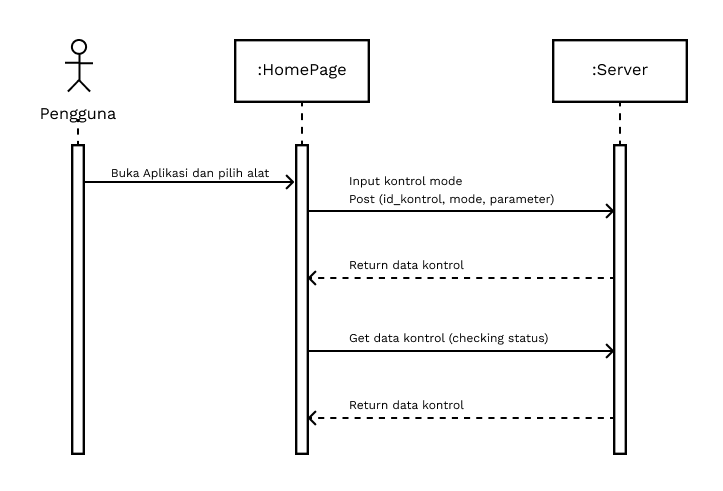
\includegraphics[width=11cm]{images/bab 4/Sequence kontrol Auto.png}
                \caption{\textit{Sequence Diagram} Melakukan Kontrol Automatis}
            \end{figure}
            \end{enumerate}
            \noindent \\\\\\\\\\\\\\\\
        \subsubsection{Pembuatan Aplikasi}
        Dalam proses pembuatan aplikasi peneliti melakukan 3 pengerjaan (1) Perancangan desain layout \textit{User Interface}, (2) Pembuatan \textit{assets} mencakup logo aplikasi, ikon sensor, dan ilustrasi kontrol, dan (3) Pengerjaan pembuatan aplikasi menggunakan \textit{framework} Flutter dengan bahasa pemrograman Dart
        \begin{enumerate}
            \item Perancangan Desain Layout \textit{User Interface}
            \begin{figure}[ht]
                \centering
                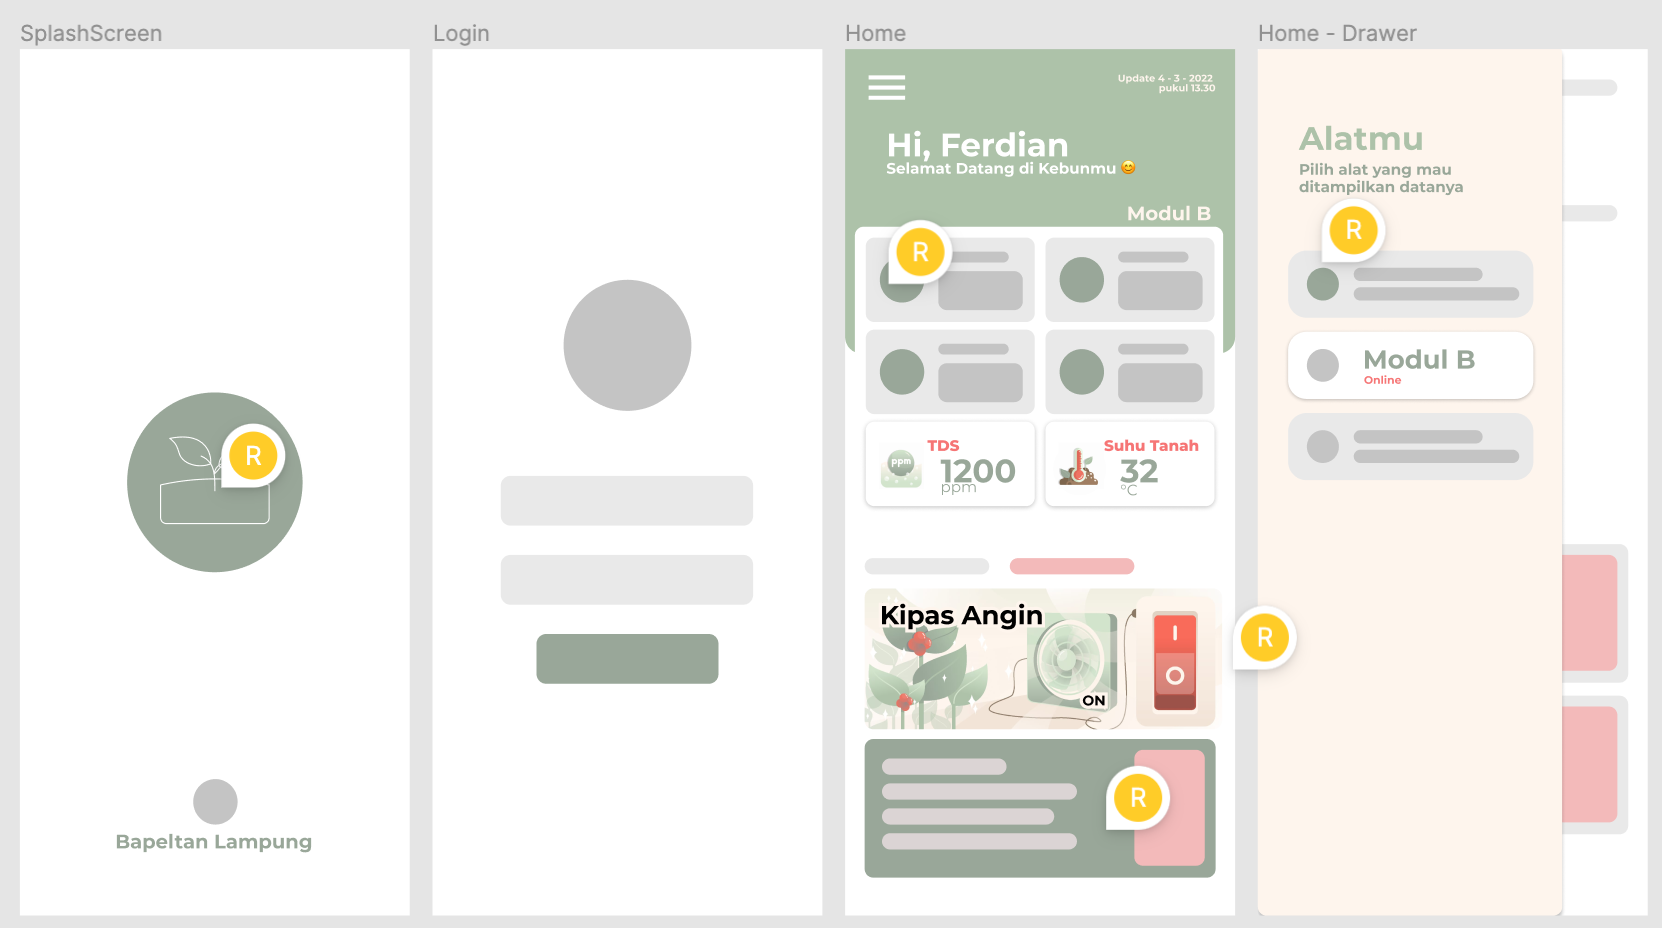
\includegraphics[width=15cm]{images/UI/summary.png}
                \caption{Rancangan layout UI}
            \end{figure}
            \vspace{10cm}
            \item Pembuatan \textit{assets}\\
            \begin{figure}[ht]
                \centering
                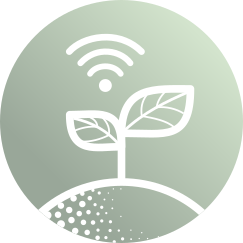
\includegraphics[width=6cm]{images/logo.png}
                \caption{\textit{assets} Logo aplikasi}
            \end{figure}
            \noindent \\Logo aplikasi KEBUNQ yang dirancang memiliki arti sebagai berikut :
            \begin{itemize}
                \item Bentuk koin : menunjukkan bahwa aplikasi KEBUNQ dirancang untuk mendukung program \emph{low cost smart farming}
                \item Tanda sinyal : menunjukkan penggunaan aplikasi memerlukan konektivitas jaringan internet untuk melakukan pemantauan dan kontrol dari jarak jauh (\emph{online apps})
                \item Tanaman : menunjukkan bahwa aplikasi KEBUNQ berhubungan erat dan tidak lepas dengan tanaman dalam penggunaannya
                \item pijakan tanaman dan bulatan-bulatan kecil : mewakilkan banyaknya unsur yang dapat kita pantau melalui aplikasi KEBUNQ.\\\\
            \end{itemize}
            \begin{figure}[ht]
                \centering
                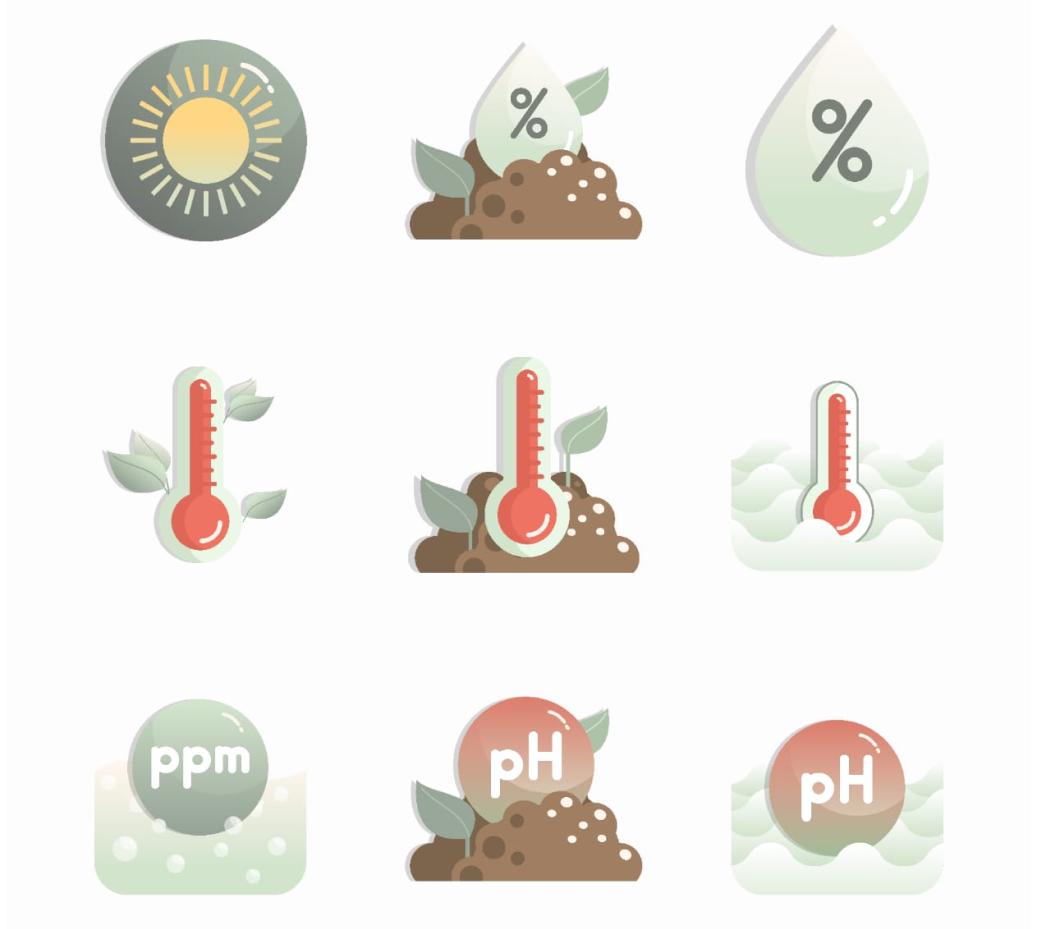
\includegraphics[width=7cm]{images/UI/ikon.png}
                \caption{\textit{assets} Ikon Sensor}
            \end{figure}
            \begin{figure}[ht]
                \centering
                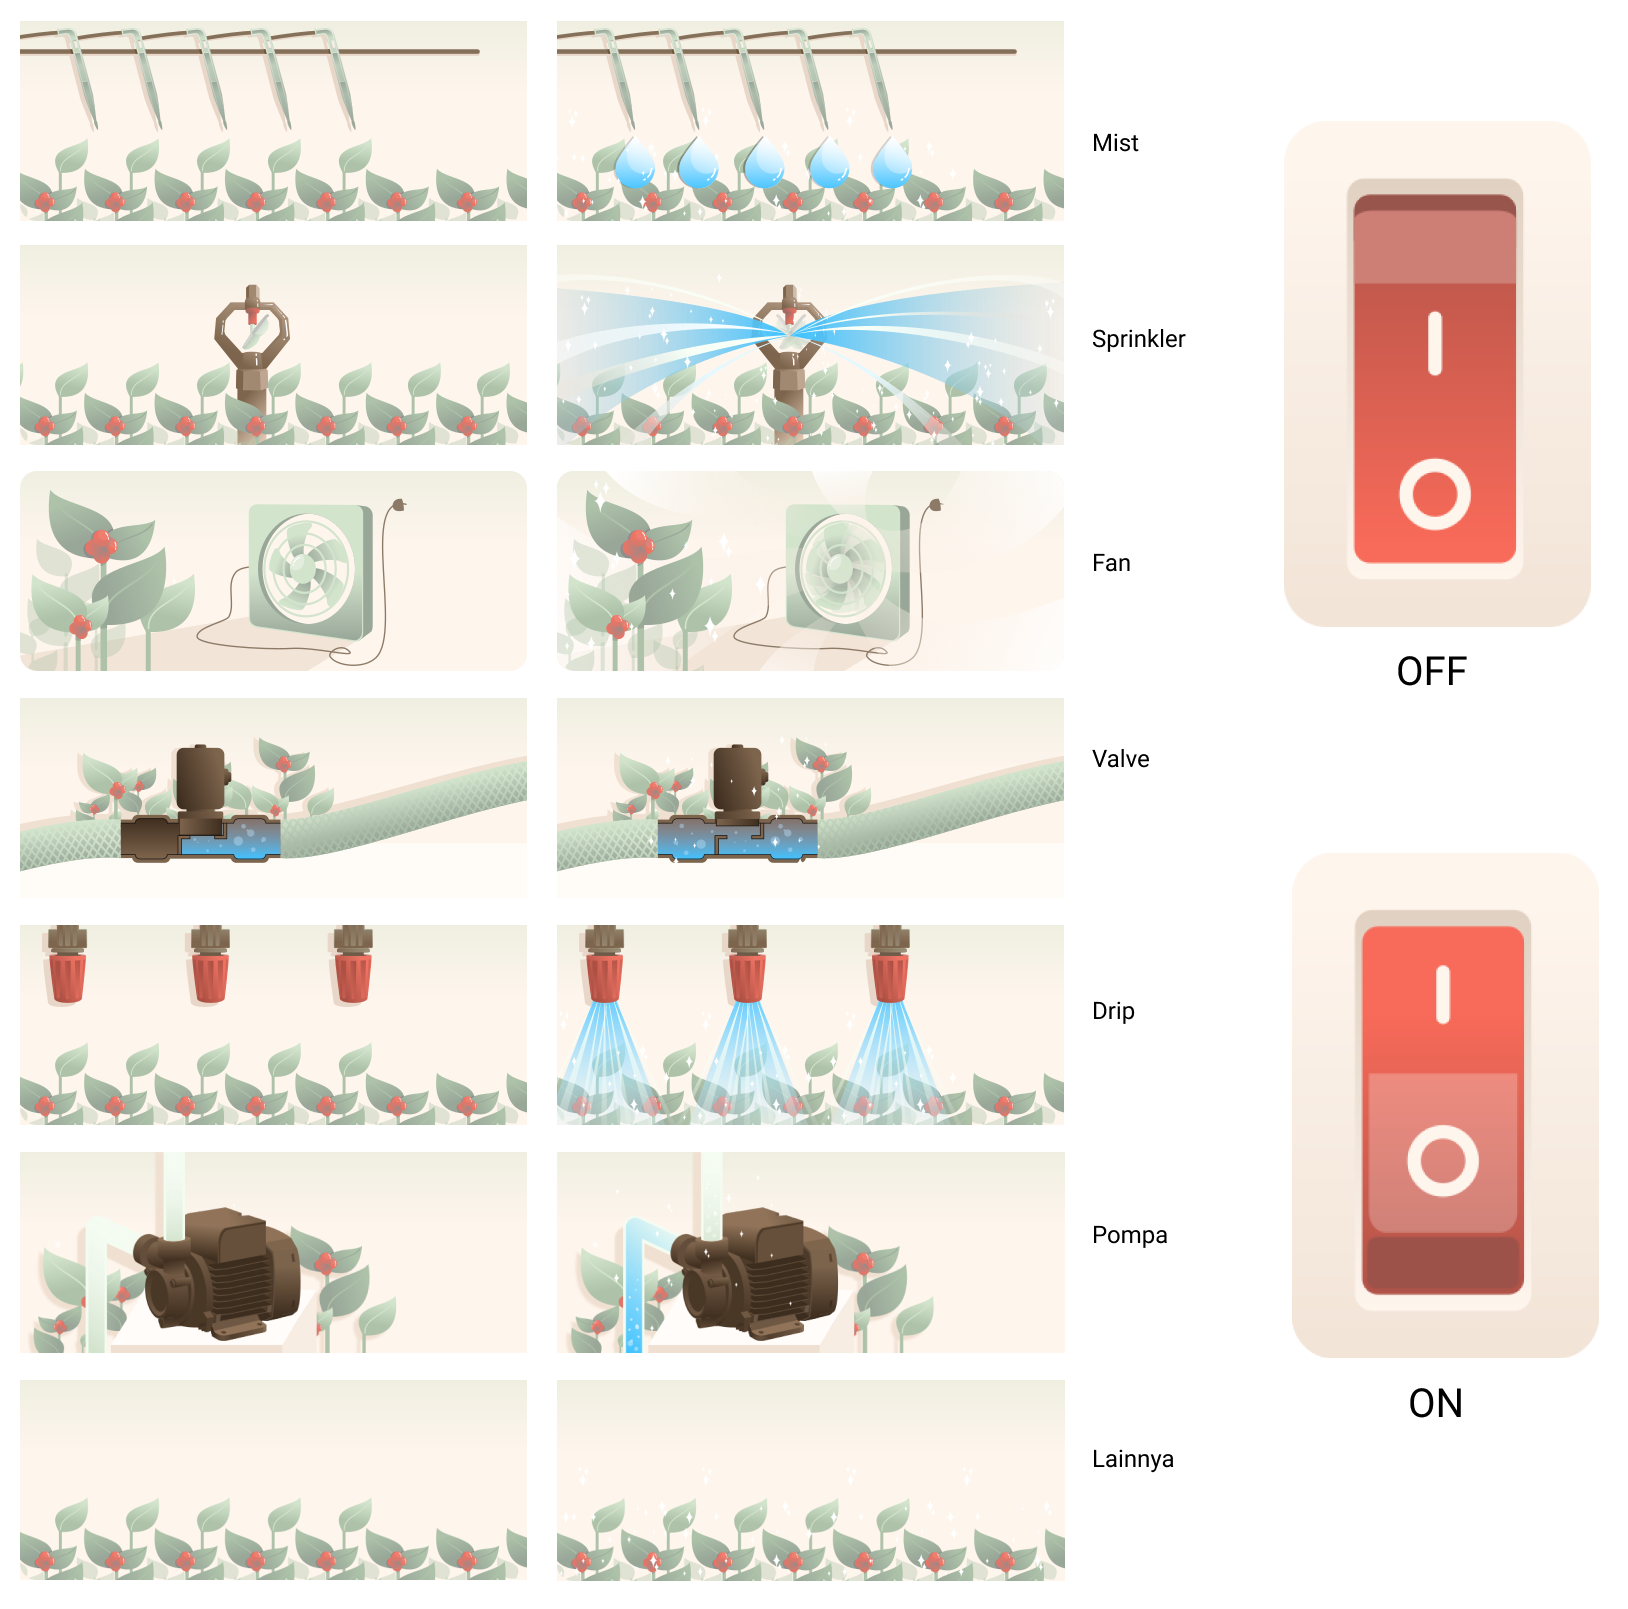
\includegraphics[width=7cm]{images/UI/Frame 1.png}
                \caption{\textit{assets} Kontrol}
            \end{figure}
            \noindent \\\\\\\\\\\\\\\\\\Pembuatan \emph{assets} logo, ikon dan ilustrasi bertujuan untuk meningkatkan kemudahan pengguna dalam menggunakan aplikasi KEBUNQ dan menjadikan KEBUNQ sebagai aplikasi yang unik dengan menggunakan \emph{assets} yang orisinil khusus didesain dan digunakan pada aplikasi KEBUNQ. \\
            \item Pembuatan Aplikasi\\
            Implementasi dari perancangan aplikasi KEBUNQ
            \begin{itemize}
                \item Halaman \emph{Splash Screen}\\
                Merupakan halaman pertama yang dilihat dengan hitungan waktu beberapa detik. Pada aplikasi KEBUNQ, \emph{splash screen} dibuat dengan sedikit implementasi gerak animasi dan mencantumkan logo KEBUNQ dan BPP Lampung.
                Halaman \emph{Splash Screen} dapat dilihat pada Gambar 4.12
                \begin{figure}[ht]
                    \centering
                    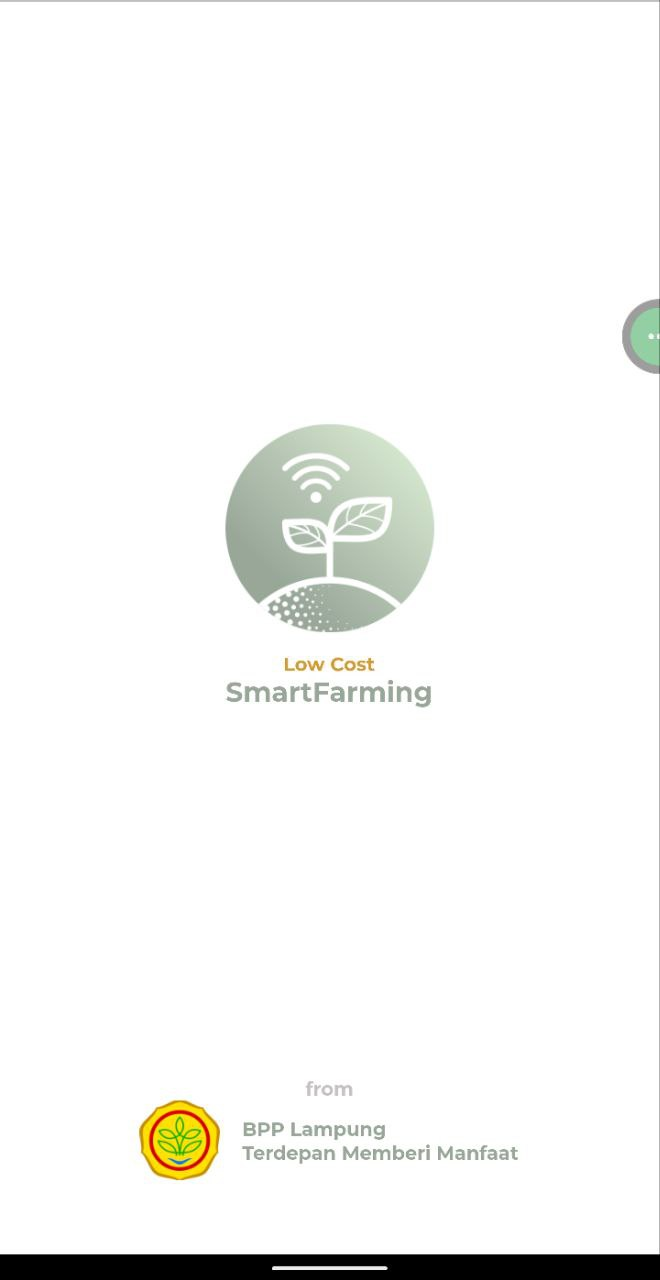
\includegraphics[width=3cm]{images/bab 4/splash.jpeg}
                    \caption{Tampilan \emph{Splash Screen}}
                \end{figure}

                \item Halaman \emph{Login}\\
                Halaman \emph{login} berupa formulir \emph{login} yang diharuskan untuk diisi dengan benar supaya kemudian pengguna dapat menggunakan fitur utama aplikasi KEBUNQ. Halaman login menampilkan \emph{field username} dan \emph{password}.
                Dalam proses \emph{login} dilakukan pemeriksaan data apakah data yang dimasukkan sesuai dengan \emph{database} atau tidak. Jika ada maka aplikasi KEBUNQ akan menampilkan halaman \emph{Home} dan menampilkan data yang dimiliki oleh pengguna. \
                Halaman \emph{login} dapat dilihat pada Gambar 4.13
                \begin{figure}[ht]
                    \centering
                    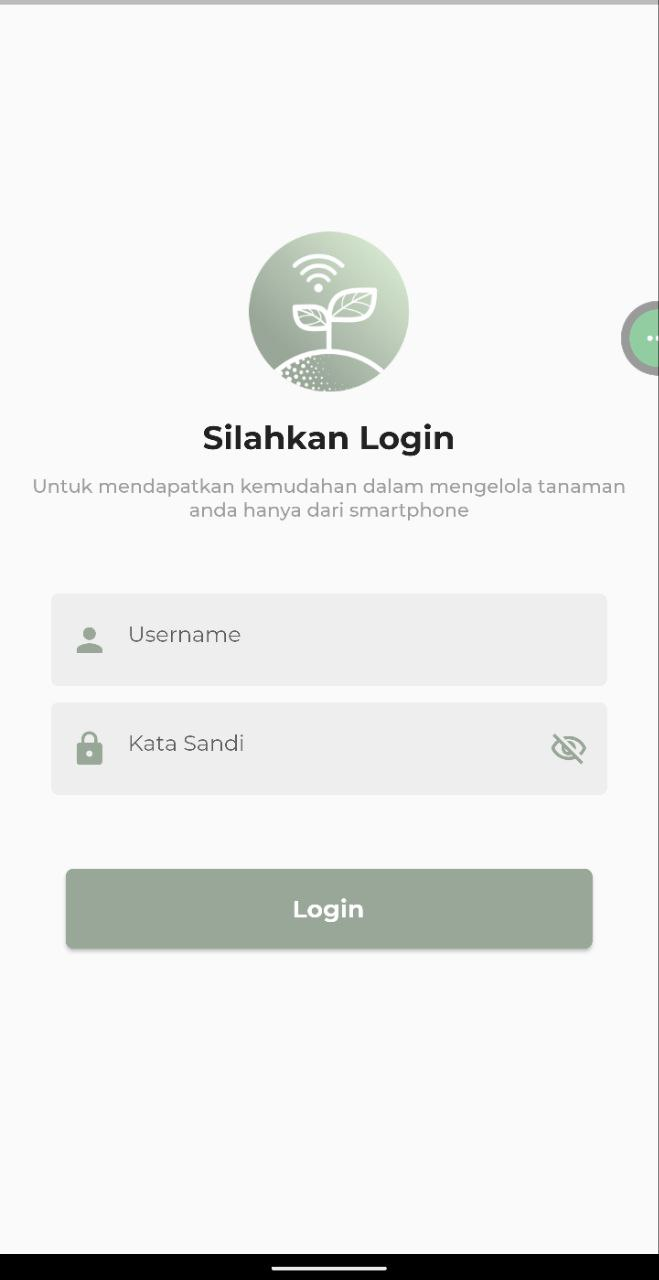
\includegraphics[width=3cm]{images/bab 4/login.jpeg}
                    \caption{Tampilan Halaman \emph{Login}}
                \end{figure}
                \vspace{10cm}
                \item Halaman \emph{Home}\\
                Halaman \emph{Home} merupakan halaman utama yang digunakan pengguna untuk melihat data sensor dan kontrol yang ada. Pengguna dapat melakukan kontrol atau kendali dengan cara menyalakan atau mematikan kontrol maupun memberikan \emph{setting} automatis pada kontrol yang dipilih.
                Halaman \emph{Home} dapat dilihat pada Gambar 4.14
                \begin{figure}[ht]
                    \centering
                    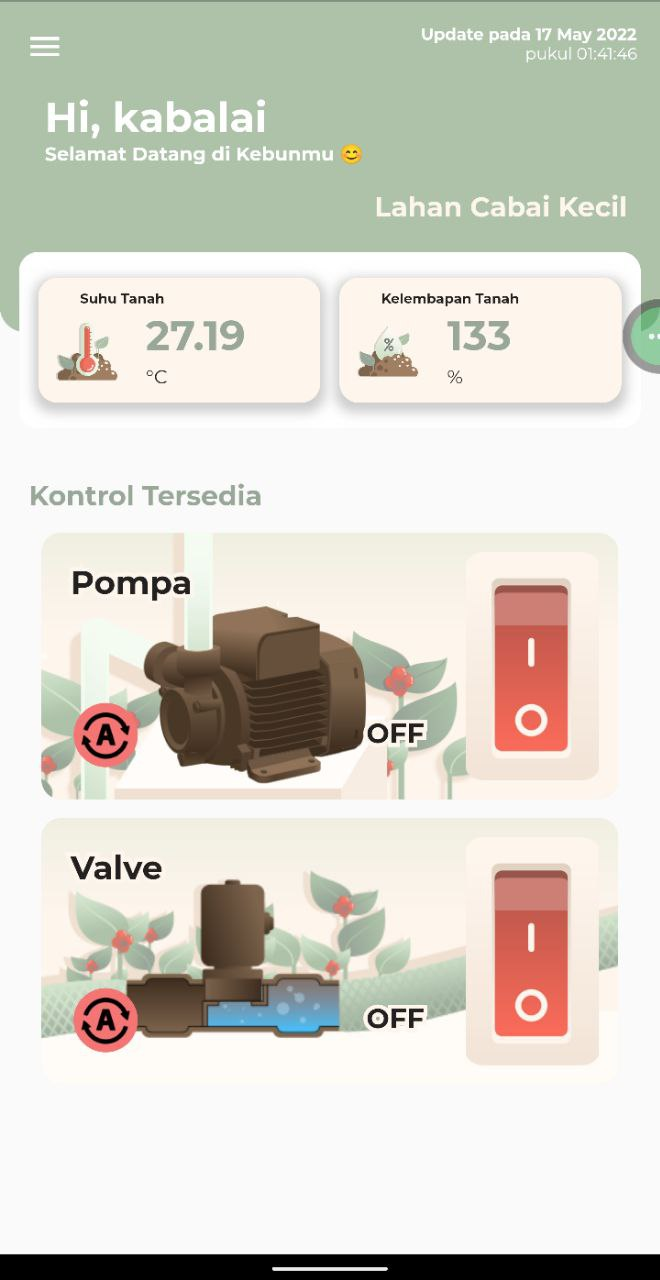
\includegraphics[width=3cm]{images/bab 4/home.jpeg}
                    \caption{Tampilan Halaman \emph{Home}}
                \end{figure}
                \newline
                \item \emph{Drawer}\\
                \emph{Drawer} merupakan bagian tampilan Menu yang terdapat pada halaman \emph{Home} ketika diklik/disentuh. Menu \emph{drawer} berisikan \emph{list} alat yang tersedia pada akun pengguna. Pada \emph{list} alat tersebut terdapat nama alat dan status keadaan alat sekarang apakah \emph{online} (keadaan nyala) atau \emph{offline} (keadaan mati).
                Tampilan menu \emph{drawer} dapat dilihat pada Gambar 4.15
                \begin{figure}[ht]
                    \centering
                    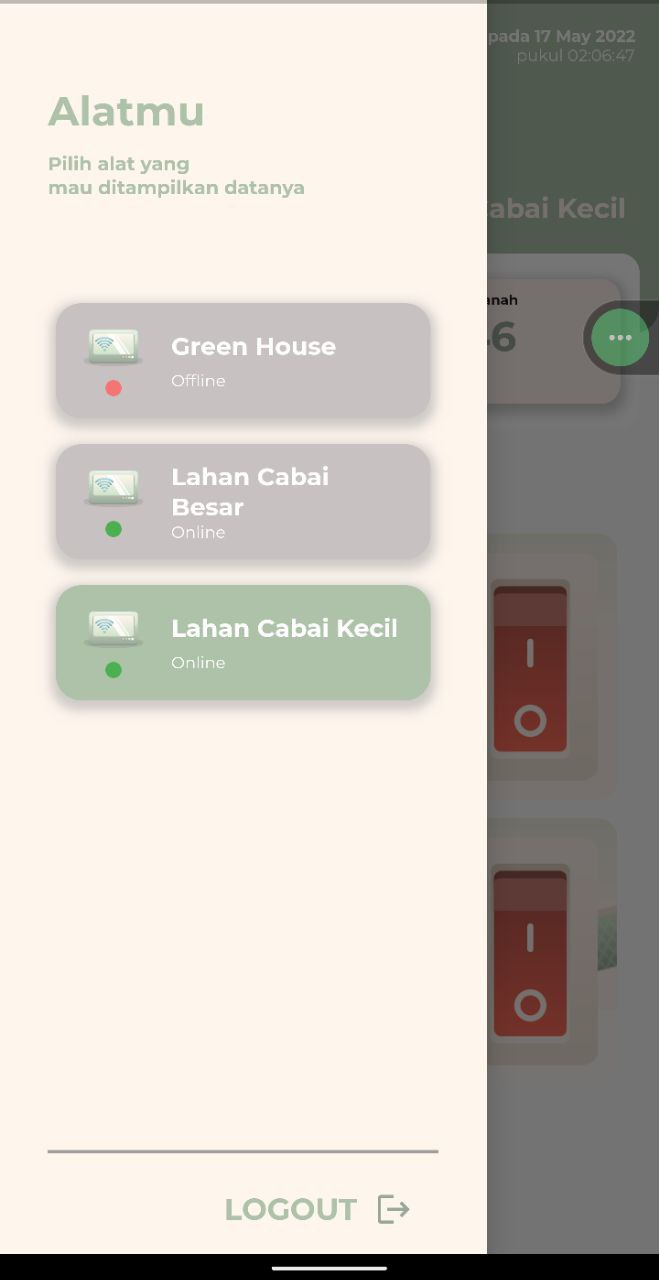
\includegraphics[width=3cm]{images/bab 4/drawerr.jpeg}
                    \caption{Tampilan Menu \emph{Drawer}}
                \end{figure}
                \item Tampilan \emph{Loading}
                Tampilan \emph{loading} merupakan tampilan yang muncul membentuk \emph{shimmer} pada layout yang dibuat ketika aplikasi KEBUNQ menunggu \emph{loading request} data dari API.
                Tampilan \emph{loading} dapat dilihat pada Gambar 4.16 
                \begin{figure}[ht]
                    \centering
                    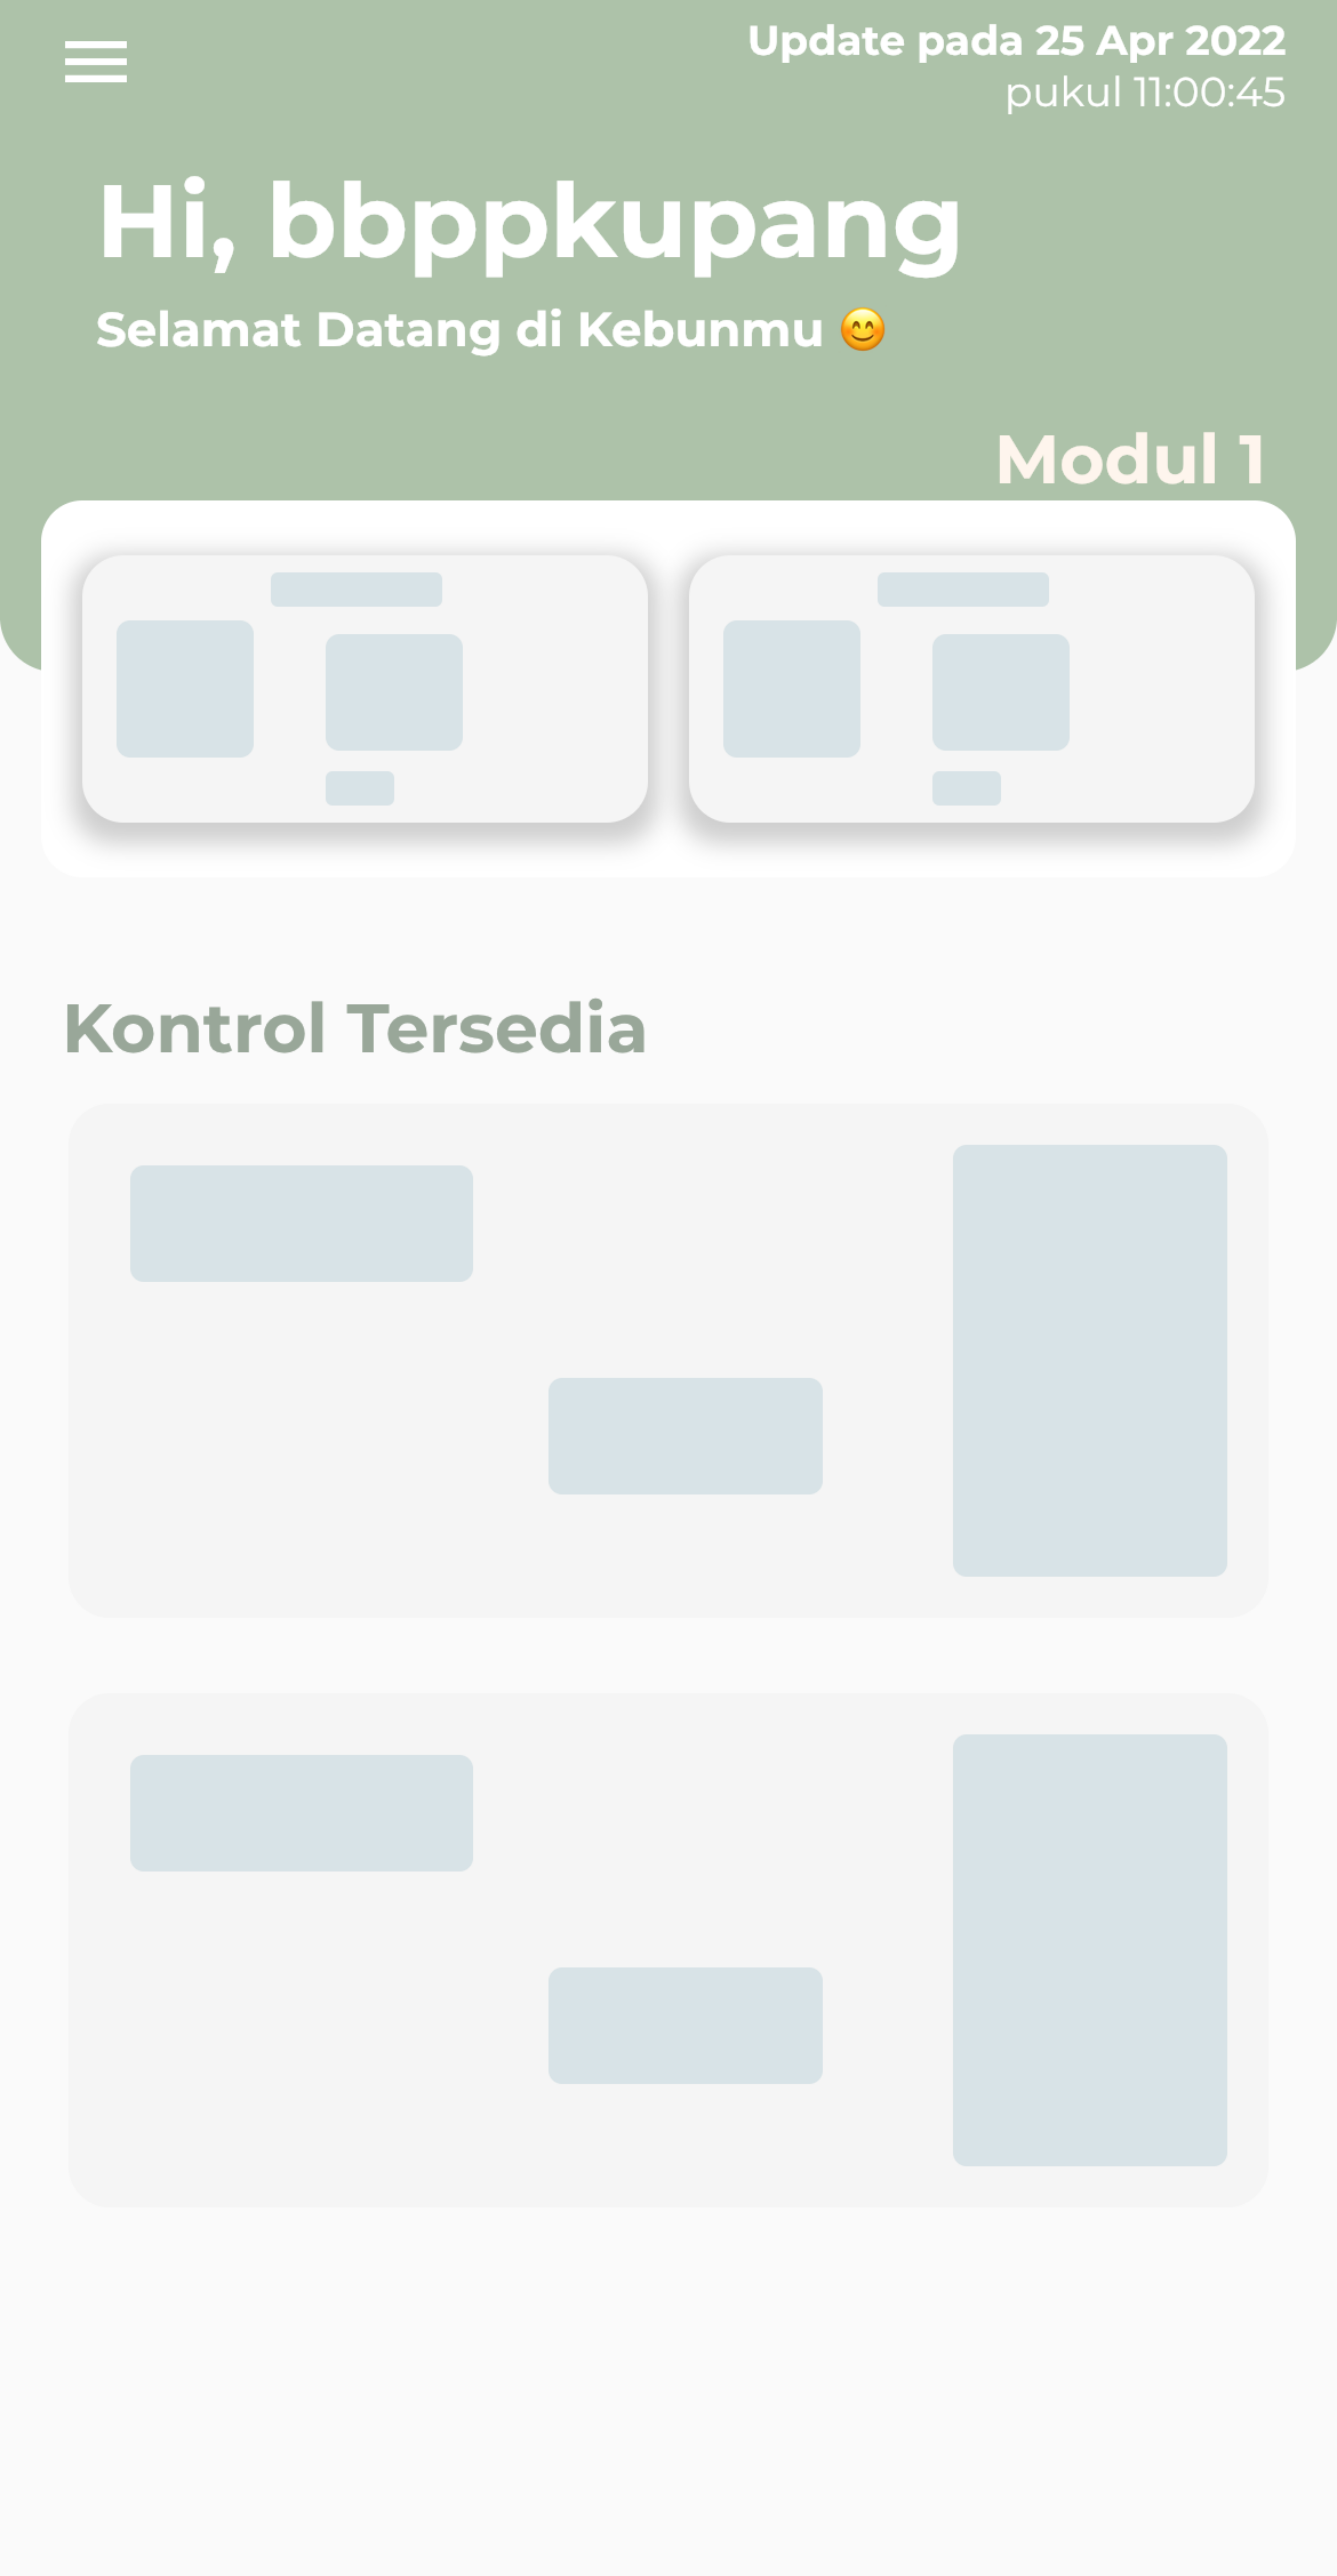
\includegraphics[width=3cm]{images/bab 4/ui-loading.png}
                    \caption{Tampilan \emph{Loading}}
                \end{figure}

            \end{itemize}
        \end{enumerate}

            \subsubsection{Pengujian dan Pergantian}
            Pada \emph{testing} aplikasinya menggunakan \emph{black box testing} untuk mencari tahu apakah aplikasi 
            sudah seperti yang dirapkan atau belum. Berikut beberapa tes yang dilakukan dapat dilihat pada Tabel 4.1 dan Tabel 4.2
            \begin{itemize}
                \item Pengujian Halaman \emph{Login}
                \begin{table}[ht]
                    \centering
                    \caption{Pengujian Halaman \emph{Login}}
                    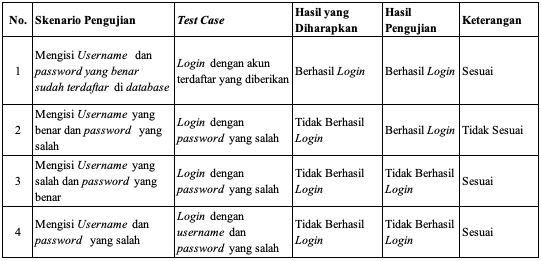
\includegraphics[width=12cm]{images/bab 4/fungsional-login.png}\\
                    \end{table}
                \item Pengujian Halaman \emph{Home}
                \begin{table}[ht]
                    \centering
                    \caption{Pengujian Halaman \emph{Home}}
                    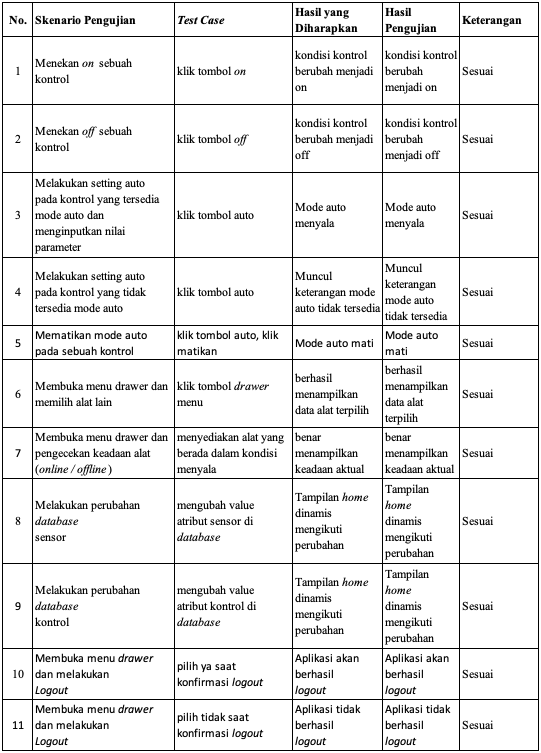
\includegraphics[width=11cm]{images/bab 4/fungsional-home.png}\\
                    \end{table}
            \end{itemize}
           
% \begin{table}[ht]
% \centering
% \caption{Permasalahan dan Solusinya}
% \begin{tabular}{|>{\raggedright}p{5cm}|p{2.5cm}|>{\raggedright}p{5cm}|}
%  \hline
%  \multicolumn{1}{|c}{\bfseries Masalah} & \multicolumn{1}{|c|}{\bfseries Aktor} & \multicolumn{1}{c|}{\bfseries Solusi} \\ 
%   \hline
% \begin{enumerate}
%    	\item Masalah masalah masalah Masalah masalah masalah Masalah masalah masalah Masalah masalah masalah.
%    	\item Masalah masalah masalah Masalah masalah masalah Masalah masalah masalah Masalah masalah masalah.
%    	\item Masalah masalah masalah Masalah masalah masalah Masalah masalah masalah Masalah masalah masalah.
%    \end{enumerate} &
%    \begin{enumerate}
%   	\item Aktor 1
%   	\item Aktor 2
%   \end{enumerate} &
%   \begin{enumerate}
%   \item Solusi solusi solusi Solusi solusi solusi Solusi solusi solusi Solusi solusi solusi Solusi solusi solusi.
%   \item Solusi solusi solusi Solusi solusi solusi Solusi solusi solusi Solusi solusi solusi Solusi solusi solusi.
%   \item Solusi solusi solusi Solusi solusi solusi Solusi solusi solusi Solusi solusi solusi Solusi solusi solusi.
%   \end{enumerate}
%      \tabularnewline
%   \hline
%  \end{tabular}
% \end{table}
        \vspace{1cm}
        \subsection{Uji Lapangan}
        Pada uji lapangan selain mengamati jalannya aplikasi sekaligus dilakukan pengujian UAT untuk mengetahui tingkat penerimaan pengguna dalam menggunakan aplikasi KEBUNQ.
        Setelah data kuesioner dikumpulkan kemudian dilakukan perhitungan persentase dengan cara mengalikan jumlah setiap pilihan jawaban 
        dengan 100 kemudian dibagi dengan jumlah responden. Persentase dapat dihitung dengan menggunakan rumus:
        \begin{equation}
            P = \frac{f}{n} \times 100\%
         \end{equation}
         \noindent Keterangan :
         \\P = Persentase
         \\n = Jumlah responden
         \\f = Frekuensi jawaban\\
         \begin{table}[ht]
            \centering
            \caption{Kuesioner}
            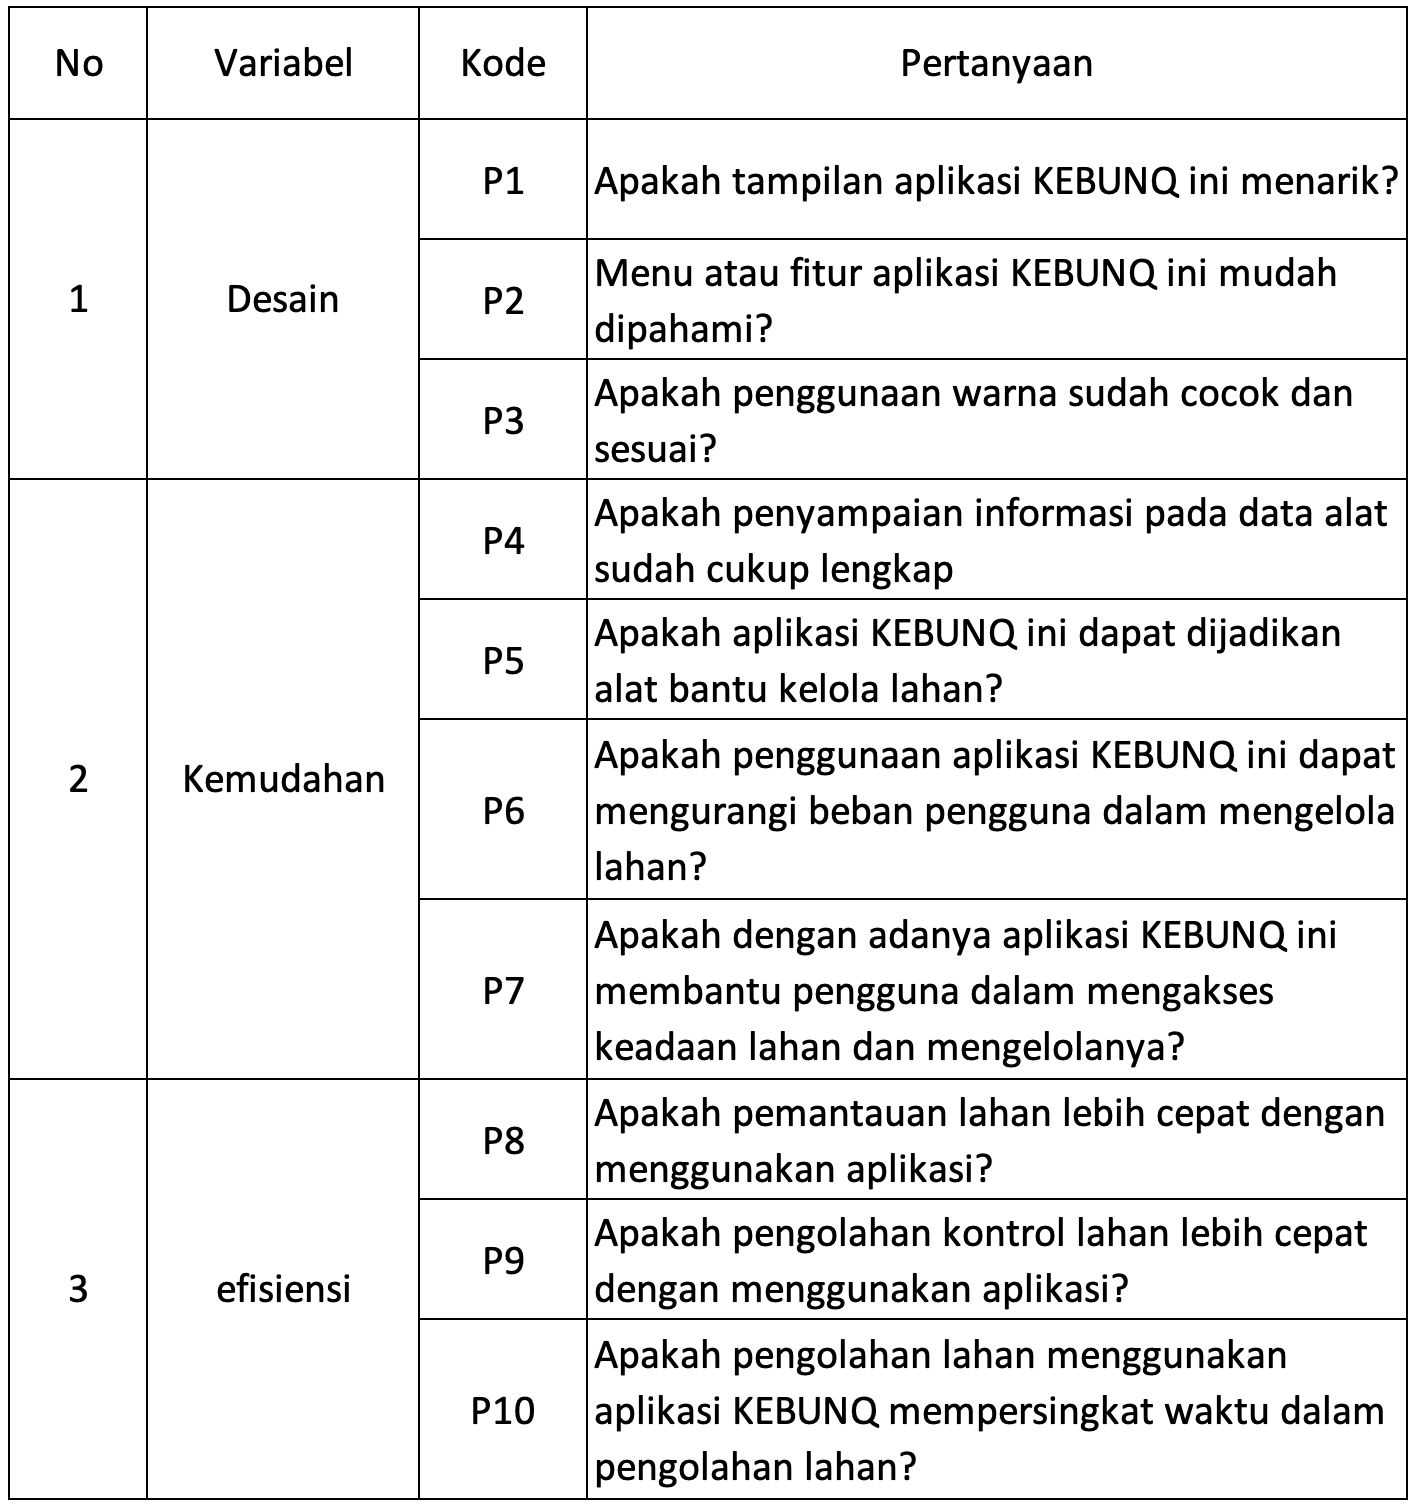
\includegraphics[width=11cm]{images/bab 4/uat.png}\\
            \end{table}
       \newline \noindent Hasil kuesioner yang dilakukan dijumlahkan berdasarkan setiap jawaban dapat dilihat pada tabel 4.4, berikut:\\
        \begin{table}[ht]
            \centering
            \caption{Kuesioner}
            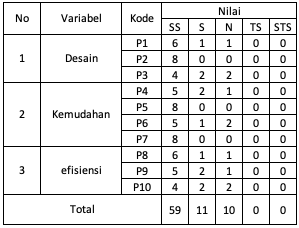
\includegraphics[width=8cm]{images/bab 4/hitungan.png}\\
            \end{table}
            \newline \noindent \\\\\\\\
            \vspace{5cm}
            \noindent \\Dari data tertera pada Tabel 4.4, dilakukan perhitungan dengan pemberian bobot pada total setiap jawaban.
            Perhitungan pembobotan dapat dilihat sebagai berikut:
            \begin{itemize}
                \item Jumlah skor responden Sangat Setuju (SS) = 59 x 5 = \textbf{295}
                \item Jumlah skor responden Setuju (S)  = 11 x 4 = \textbf{44}
                \item Jumlah skor responden Netral (N)  = 10 x 3 = \textbf{30}
                \item Jumlah skor responden Tidak Setuju (TS)  = 0 x 2 = \textbf{0}
                \item Jumlah skor responden Sangat Tidak Setuju (STS)  = 0 x 1 = \textbf{0}
            \end{itemize}
            Maka didapat jumlah total dari pemberian bobot adalah \textbf{369}\\
            Hasil jawaban dari 8 responden tersebut kemudian dilakukan perhitungan nilai terendah dan tertinggi seperti berikut:
            \begin{itemize}
                \item Nilai terendah = 8 x 10 x 1 = \textbf{80}
                \item Nilai tertinggi = 8 x 10 x 5 = \textbf{400}
             \end{itemize}
             Hasil perhitungan nilai tertinggi yang didapat adalah 400. Kemudian dilakukan perhitungan persentase menggunaan persamaan sebelumnya, sebagai berikut:
             \begin{equation}
                P = \frac{369}{400} \times 100\% = 92,2\%
             \end{equation}
             Berdasarkan perhitungan di atas, didapatkan bahwa tingkat penerimaan terhadap aplikasi KEBUNQ terletak pada rentang 81\% - 100\%, 
             masuk dalam kategori nilai kesimpulan sangat kuat sesuai dengan yang dikemukakan oleh Riduwan dalam referensi \cite{kuantitatif}, dengan nilai perhitungan persentase
             92,2\%, yang berarti aplikasi KEBUNQ ini dapat diterima oleh pengguna. Hasil persentase tersebut dapat dilihat pada skala penilaian pada Gambar 4.17 berikut ini:
             \begin{figure}[ht]
                \centering
                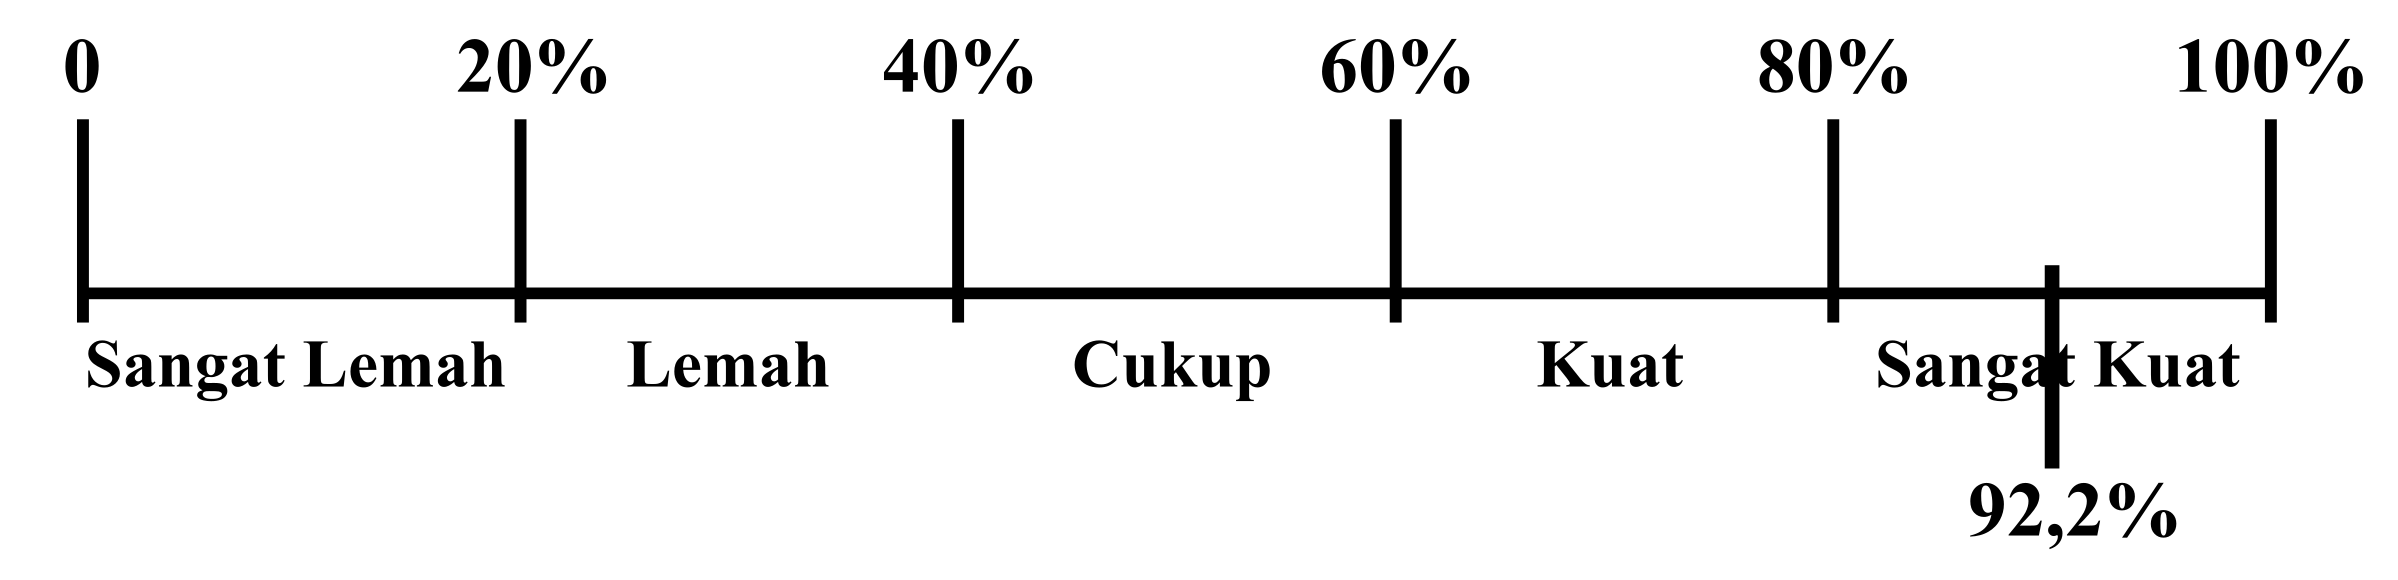
\includegraphics[width=8cm]{images/bab 4/persentase.png}
                \caption{Skala penilaian}
            \end{figure}


   
        \section{Pembahasan}
        Pada tahap observasi didapatkan jenis-jenis sensor dan kontrol yang akan dimasukkan pada penentuan bagaimana aplikasi dirancang dan dibuat. Pada tahap pembuatan aplikasi KEBUNQ, peneliti menggunakan \emph{framework Flutter} dengan bahasa pemrograman \emph{Dart}. Dalam penelitian ini dilakukan dua metode pengujian yaitu \emph{black box testing} dan UAT. Pada pengujian \emph{black box} terdapat satu hasil yang tidak sesuai dengan yang diharapkan, yaitu pada
        pengujian halaman login saat melakukan pengisian \emph{username} yang benar dan \emph{password} yang salah, setelah dilakukan pengecekan permasalahannya terdapat pada API login yang diterima peneliti 
        belum melakukan validasi password dan hanya melakukan validasi pada \emph{username}. Selanjutnya pada pengujian UAT, didapatkan hasil persentase sebesar 92,2\% yang menunjukkan penerimaan pengguna yang sangat kuat.
         

    








    \end{justify}




    
\end{flushleft}

\newpage